%
% LaTeX report template
%
\documentclass[a4paper,10pt]{article}
\usepackage{titlesec}
\usepackage{graphicx}
\usepackage{amsmath}
\usepackage[english]{babel}
\usepackage{hyperref}
\usepackage{tikz}
\usepackage{amssymb}% http://ctan.org/pkg/amssymb
\usepackage{pifont}% http://ctan.org/pkg/pifont
\usepackage{breqn}
\usepackage[backend=biber,bibencoding=utf8, %instead of bibtex
%backend=bibtex8,bibencoding=ascii,%
language=english,%
style=numeric-comp,%
%style=authoryear-comp, % Author 1999, 2010
%bibstyle=authoryear,dashed=false, % dashed: substitute rep. author with ---
sorting=nyt, % name, year, title
maxbibnames=10, % default: 3, et al.
%backref=true,%
natbib=true]{biblatex}
\addbibresource{references.bib}

\newcommand{\cmark}{\ding{51}}%
\newcommand{\xmark}{\ding{55}}%
\usetikzlibrary{shapes,fit}
%\usepackage[latin1]{inputenc}
%
\titleclass{\subsubsubsection}{straight}[\subsubsection]

\newcounter{subsubsubsection}[subsubsection]
\renewcommand\thesubsubsubsection{\thesubsubsection.\arabic{subsubsubsection}}
\renewcommand\theparagraph{\thesubsubsubsection.\arabic{paragraph}} % optional; useful if paragraphs are to be numbered

\titleformat{\subsubsubsection}
  {\normalfont\normalsize\bfseries}{\thesubsubsubsection}{1em}{}
\titlespacing*{\subsubsubsection}
{0pt}{3.25ex plus 1ex minus .2ex}{1.5ex plus .2ex}

\makeatletter
\renewcommand\paragraph{\@startsection{paragraph}{5}{\z@}%
  {3.25ex \@plus1ex \@minus.2ex}%
  {-1em}%
  {\normalfont\normalsize\bfseries}}
\renewcommand\subparagraph{\@startsection{subparagraph}{6}{\parindent}%
  {3.25ex \@plus1ex \@minus .2ex}%
  {-1em}%
  {\normalfont\normalsize\bfseries}}
\def\toclevel@subsubsubsection{4}
\def\toclevel@paragraph{5}
\def\toclevel@paragraph{6}
\def\l@subsubsubsection{\@dottedtocline{4}{7em}{4em}}
\def\l@paragraph{\@dottedtocline{5}{10em}{5em}}
\def\l@subparagraph{\@dottedtocline{6}{14em}{6em}}
\makeatother

\setcounter{tocdepth}{3}
\setcounter{secnumdepth}{3}

\begin{document}
%
\title{Present Wrapping problem}

\author{Leonardo Calbi - leonardo.calbi@studio.unibo.it \\ Alessio Falai - alessio.falai@studio.unibo.it}

\date{\today}

\maketitle

\tableofcontents

\newpage

\section*{Foreword}
The problem is presented as: given a wrapping paper roll of a certain dimension and a list of presents, decide how to cut off pieces of paper so  that all the presents can be wrapped.

Consider that each present is described by the dimensions of the piece of paper needed to wrap it. Moreover, each necessary piece of paper cannot be rotated when cutting off, to respect the direction of the patterns in the paper.

A more general case also requires the following conditions:
\begin{itemize}
   \item Rotation of the pieces of paper is allowed
   \item There can be multiple presents of the same dimensions
\end{itemize}

\section{Introduction}
The non-overlapment requirement of \emph{PWP} links it to a specialization of the more general rectangle packing problem, in which we have a set of rectangles (our presents) of given dimensions that have to fit into a pre-determined square (the wrapping paper) of a given size.

Observing the assigned problem instances, we assume that the items will perfectly fit into the given container, without any kind of wasted space. This assumption greatly simplifies the problem, by reducing it from a minimization problem to a satisfiability one.

The following sections describe our implementation of different \emph{PWP} solutions using both Constraint Programming and Satisfiability Modulo Theory approaches.

\section{Input}
Each instance of the problem is defined by:
\begin{itemize}
   \item \texttt{n} $\longleftarrow$ number of presents to be wrapped
   \item \texttt{w\_paper} or \texttt{w} $\longleftarrow$ width of the paper roll
   \item \texttt{h\_paper} or \texttt{h} $\longleftarrow$ height of the paper roll
   \item \texttt{presents} or \texttt{p} $\longleftarrow$ list of presents dimensions, in the form $[width,height]$
\end{itemize}

To better represent equations in the following sections, \texttt{presents} is divided in two additional lists, i.e. \texttt{presents\_xs} or \texttt{px} and \texttt{presents\_ys} or \texttt{py}.

\section{Constraint Programming}
CP models are implemented with the MiniZinc language and models execution is managed by the official MiniZinc Jupyter extension, called iMiniZinc.

Following standard CP model guidelines we proceded by searching for global constraints, since they enable stronger propagation w.r.t user-defined ones, implied constraints, to allow a reduction of the search tree by pruning, channeling constraints, which can be used to gain a different point of view over the problem, symmetry-breaking constraints, that remove symmetric non-solutions from being analyzed.

In our case-study we tried different approaches, by developing different models. Some of them tend to be faster in a specific subset of instances, w.r.t. the others. In the final model, we tried to put together the different key-points of each model.

In the following subsections each and every tested constriant, along with associated decision variables, will be carefully explained.

Inserire qui roba riguardo variabili/vincoli scartati.
\subsection{Decision variables}
\subsubsection*{Bottom-left corners} \label{sec:bottom-left-corners}
This is a two-dimensional list of decision variables (\texttt{bl\_corners} or \texttt{b}), where each entry represents the bottom-left corner of a rectangle in the bounding box. Finding a satisfying assignement for this list is the main goal of this project. Moreover, the list is also used to graphically represent every instance solution.

To ease its usage two additional lists were defined (\texttt{bl\_corners\_xs} or \texttt{bx} and \texttt{bl\_corners\_ys} or \texttt{by}), by channeling over each dimension of the original list.

To reduce the search space, bottom-left corners variables domains are defined as follows:
\begin{itemize}
   \item \texttt{bl\_corners}: $0 \dots \max({h, w}) - \min({\min({px}), \min({py})})$
   \item \texttt{bl\_corners\_xs}: $0 \dots w - \min({px})$
   \item \texttt{bl\_corners\_ys}: $0 \dots h - \min({py})$
\end{itemize}

\begin{figure}[h]
   \centering
   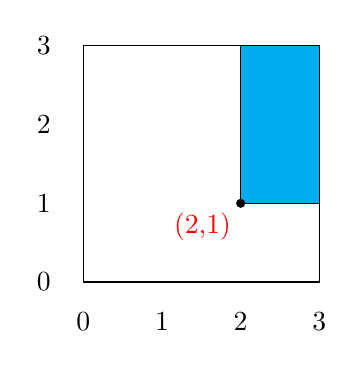
\begin{tikzpicture}
      \draw[step=1cm,black,thin] (0,0) rectangle (3,3);
      \foreach \xtick in {0,...,3} {\pgfmathsetmacro\result{\xtick * 1} \node at (\xtick,-0.5) {\pgfmathprintnumber{\result}}; }
      \foreach \ytick in {0,...,3} {\pgfmathsetmacro\result{\ytick * 1} \node at (-.5,\ytick) {\pgfmathprintnumber{\result}}; }
      \draw[fill=cyan] (2,1) rectangle (3,3);
      \draw [fill=black, thin] (2,1) circle [radius=0.05] node[below left,color=red]{(2,1)};
   \end{tikzpicture}
   \caption{Bottom-left corner example}
\end{figure}

\subsubsection*{Top-right corners}
As \nameref{sec:bottom-left-corners} but representing the top-right corner of each rectangle (\texttt{tr\_corners}). It is used to reduce the number of positions in which a rectangle can fall in, because it must be inside the bounding box.

To reduce the search space, \texttt{tr\_corners} variables domain is defined as follows: $$\min({\min({px}), \min({py})}) \dots \max({h, w})$$

\begin{figure}[h]
   \centering
   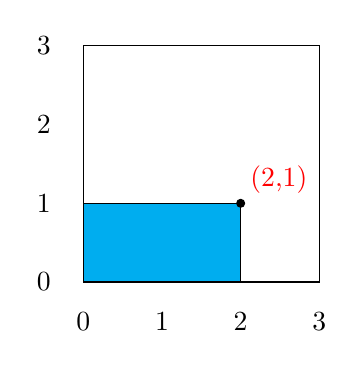
\begin{tikzpicture}
      \draw[step=1cm,black,thin] (0,0) rectangle (3,3);
      \foreach \xtick in {0,...,3} {\pgfmathsetmacro\result{\xtick * 1} \node at (\xtick,-0.5) {\pgfmathprintnumber{\result}}; }
      \foreach \ytick in {0,...,3} {\pgfmathsetmacro\result{\ytick * 1} \node at (-.5,\ytick) {\pgfmathprintnumber{\result}}; }
      \draw[fill=cyan] (0,0) rectangle (2,1);
      \draw [fill=black, thin] (2,1) circle [radius=0.05] node[above right,color=red]{(2,1)};
   \end{tikzpicture}
   \caption{Top-right corner example}
\end{figure}

\subsubsection*{Bottom-left corners values}
This is a list of decision variables representing a linearization of bottom-left corners (\texttt{bl\_corners\_values}), which uses a one-to-one mapping from each two-dimensional coordinate in the bounding box to an integer value.

The mapping operates as follows:
$$ c: (x,y) \mapsto x+(y\cdot m),$$ where $m = \max{(h,w)}$.

To reduce the search space, \texttt{bl\_corners\_values} variables domain is defined as follows: $$0 \dots c(w, h)$$

\begin{figure}[h]
   \centering
   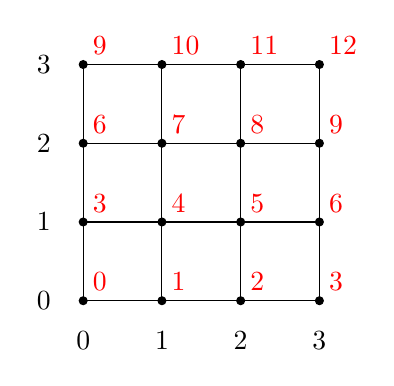
\begin{tikzpicture}
      \draw[step=1cm,black,thin] (0,0) grid (3,3);
      \foreach \xtick in {0,...,3} {\pgfmathsetmacro\result{\xtick * 1} \node at (\xtick,-0.5) {\pgfmathprintnumber{\result}}; }
      \foreach \ytick in {0,...,3} {\pgfmathsetmacro\result{\ytick * 1} \node at (-.5,\ytick) {\pgfmathprintnumber{\result}}; }
      \foreach \x in {0,...,3} {\foreach \y in {0,...,3} {\draw [fill=black, thin] (\x,\y) circle [radius=0.05] node[above right,color=red] {\pgfmathparse{\x+\y*3} \pgfmathprintnumber{\pgfmathresult}};}}
   \end{tikzpicture}
   \caption{Example of 2D-coordinates linearization in a 3 by 3 box}
\end{figure}

\subsection{Constraints}
The constraints described below, divided by scope, are presented at the top of each section with a simple schema depicting their evolution throughout different models.
The following is a legend explaining how constraints advancement is achieved:
\begin{itemize}
   \item \texttt{A[x]}: Constraint \texttt{A} has been introduced in model number \texttt{x}
   \item \texttt{A[x]} $\rightarrow$ \texttt{B[y]}: Constraint \texttt{A} was removed in favor of \texttt{B}, in model \texttt{y}
   \item \texttt{A[x]} $\rightarrow$ \xmark: Constraint \texttt{A} has not been carried over to models \texttt{x + 1, \dots}
\end{itemize}
Model numbers are related to the organization inside the Jupyter notebook.

\subsubsection{Non-overlapment}
\begin{itemize}
   \item \nameref{sec:presents-cannot-overlap} $\rightarrow$ \nameref{sec:diffnk}
   \item \nameref{sec:different-bl-corners}
\end{itemize}

\subsubsubsection{Presents cannot overlap [1]} \label{sec:presents-cannot-overlap}
The idea behind this simple constraint is, given a rectangle, to avoid the existance of areas of overlap with every other rectangle.
\begin{gather*}
   \max({bx_{i}, bx_{j}}) \geq \min({bx_{i} + px_{i}, bx_{j} + px_{j}}) \\
   \vee \\
   \max({by_{i}, by_{j}}) \geq \min({by_{i} + py_{i}, by_{j} + py_{j}}) \\
   \forall{i, j \mid j > i}
\end{gather*}

The described constraint has been observed to be efficient enough for relatively small instances of the problem, while already suffering to position rectangles in a $17 \times 17$ bounding box. Results are justified by the disjunctive nature of the constraint, which implies an higher burden in the propagation phase.

\subsubsubsection{Global \texttt{diffn\_k} [3]} \label{sec:diffnk}
The \texttt{diffn\_k} global constraint is defined by the official MiniZinc documentation \cite{minizinc} as follows: \\
\emph{Constrains k-dimensional boxes to be non-overlapping. For each box i and dimension j, box\_posn[i, j] is the base position of the box in dimension j, and box\_size[i, j] is the size in that dimension. Boxes whose size is 0 in any dimension still cannot overlap with any other box.}
\begin{verbatim}
   constraint diffn_k(bl_corners, presents);
\end{verbatim}
Being a global constraint it gives a stronger propagation and a more efficient search w.r.t to \nameref{sec:presents-cannot-overlap}, allowing us to solve bigger instances, up to a $23 \times 23$ bounding box.

It's also notable, as described by \cite{sweep}, that \texttt{diffn\_k} is an onerous constraint. In \cite{sweep} it accounts for 30 to 80\% of the total running time in an implementation of \emph{PSP (Perfect Square Packing)} problem, which is very much related to \emph{PWP}.
\subsubsubsection{Global \texttt{all\_different} [2]} \label{sec:different-bl-corners}
The \texttt{all\_different} global constraint asserts that every variable has a different value assigned to it.

In our models it is used w.r.t \texttt{bl\_corners\_values} to ensure that every present has different \texttt{bl\_corners}. The choice of the constrained variables is related to their one-dimensional nature, which guarantees compatibility with MiniZinc's implementation of \texttt{all\_different}.
\begin{verbatim}
   constraint alldifferent(bl_corners_values);
\end{verbatim}
\subsubsection{Containment}
\begin{itemize}
   \item \nameref{sec:reduce-presents-domains}
   \item \nameref{sec:areas-summation}
\end{itemize}

\subsubsubsection{Reduce presents domains [1]} \label{sec:reduce-presents-domains}
\subsubsubsection{Areas summation [4]} \label{sec:areas-summation}

\subsubsection{Positioning}
\begin{itemize}
   \item \nameref{sec:present-at-origin}
   \item \nameref{sec:intervals-approach} $\rightarrow$ \xmark
   \item \nameref{sec:anchor-points-v1} $\rightarrow$ \nameref{sec:anchor-points-v2}$\rightarrow$ \xmark
\end{itemize}

\subsubsubsection{Global \texttt{count\_eq} [2]} \label{sec:present-at-origin}
\subsubsubsection{Intervals approach [5]} \label{sec:intervals-approach}
\subsubsubsection{Anchor points [5]} \label{sec:anchor-points-v1}
\subsubsubsection{Anchor points [6]} \label{sec:anchor-points-v2}

\subsubsection{Stacking}
\begin{itemize}
   \item \nameref{sec:cumulative}
   \item \nameref{sec:stack-two} $\rightarrow$ \nameref{sec:column-stacking}
\end{itemize}

\subsubsubsection{Global \texttt{cumulative} [3]} \label{sec:cumulative}
\subsubsubsection{Column stacking by two [4]} \label{sec:stack-two}
\subsubsubsection{General column stacking [5]} \label{sec:column-stacking}

\subsubsection{Symmetry breaking}
\begin{itemize}
   \item \nameref{sec:biggest-lower-left} $\rightarrow$ \nameref{sec:areas-ordering}
   \item \nameref{sec:width-ordering} $\rightarrow$ \xmark
\end{itemize}

\subsubsubsection{Biggest rectangle in lower left quadrant [4]} \label{sec:biggest-lower-left}
\subsubsubsection{Ordering by areas [6]} \label{sec:areas-ordering}
\subsubsubsection{In-column ordering by width [4]} \label{sec:width-ordering}


\subsection{Models}

\subsubsection*{Search strategy}

\LaTeX is a very powerful tool when it comes to typesetting of
mathematical equations. The quality of the output is extremely
high and hardly matched by other word processors. It takes little
time with {\LaTeX\,}  to learn how to handle
even complicated mathematical expressions.
\begin{eqnarray}
   \sigma_0 & = & \frac{\pi}{\sqrt{8}}
   \frac{1}{ \tau_{\mathrm{ff}}} \\
   K        & = & \frac{\sqrt{32}}{\pi} \frac{1}{\delta}
   \frac{ \tau_{\mathrm{ff}} }
   { \tau_{\mathrm{co}} }\,;
\end{eqnarray}

\LaTeX\, uses a simple and convenient system for assigning numbered labels
to equations and other objects (figures, tables, etc\ldots) and for referring
to them. After having edited the source file and rearranged the position of
the equations, \LaTeX\, will  change labels and references
consistently throughout the text (if you did the things right of
course\ldots)

Examples of text containing mathematical expressions and equations:
\[
   \begin{array}{lp{0.8\linewidth}}
      M_{r}           & mass internal to the radius $r$     \\
      m               & mass of the zone                    \\
      r_0             & unperturbed zone radius             \\
      \rho_0          & unperturbed density in the zone     \\
      T_0             & unperturbed temperature in the zone \\
      L_{r0}          & unperturbed luminosity              \\
      E_{\mathrm{th}} & thermal energy of the zone
   \end{array}
\]

\noindent

\begin{equation}
   \tau_{\mathrm{co}} = \frac{E_{\mathrm{th}}}{L_{r0}} \,,
\end{equation}


\begin{equation}
   \tau_{\mathrm{ff}} =
   \sqrt{
      \frac{3 \pi}{32 G} \frac{4\pi r_0^3}{3 M_{\mathrm{r}}}
   }\,,
\end{equation}


\begin{displaymath}
   \nabla_{\mathrm{ad}} = \left( \frac{ \partial \ln T}
   { \partial\ln P} \right)_{S} \, , \;
   \chi^{}_T       = \left( \frac{ \partial \ln P}
   { \partial\ln T} \right)_{\rho} \, , \;
   \kappa^{}_{T}   = \left( \frac{ \partial \ln \kappa}
   { \partial\ln T} \right)_{T}
\end{displaymath}

\begin{eqnarray}
   \frac{\pi^2}{8} \frac{1}{\tau_{\mathrm{ff}}^2}
   ( 3 \Gamma_1 - 4 )
   & > & 0 \label{ZSDynSta} \\
   \frac{\pi^2}{\tau_{\mathrm{co}}
      \tau_{\mathrm{ff}}^2}
   \Gamma_1 \nabla_{\mathrm{ad}}
   \left[ \frac{ 1- 3/4 \chi^{}_\rho }{ \chi^{}_T }
      ( \kappa^{}_T - 4 )
      + \kappa^{}_P + 1
      \right]
   & > & 0 \label{ZSSecSta} \\
   \frac{\pi^2}{4} \frac{3}{\tau_{ \mathrm{co} }
      \tau_{ \mathrm{ff} }^2
   }
   \Gamma_1^2 \, \nabla_{\mathrm{ad}} \left[
      4 \nabla_{\mathrm{ad}}
      - ( \nabla_{\mathrm{ad}} \kappa^{}_T
      + \kappa^{}_P
      )
      - \frac{4}{3 \Gamma_1}
      \right]
   & > & 0   \label{ZSVibSta}
\end{eqnarray}

\subsection{Results}
In \LaTeX\, You can enter text \texttt{verbatim}: that means that
\LaTeX\, will print it exactly as you enter it in the source file. The
output resembles closely the one from old typewriters and it
is usually good to print out portions of computer code:

\begin{verbatim}
        PROGRAM area
        REAL base, height, area
        PRINT *,'Enter the values for the base and height of a triangle.'
        READ *, base, height
        area = (1.0/2.0) * base * height
        PRINT *,'The area of a triangle with base ', base
        PRINT *,'and height ', height,' is ', area
        STOP
        END
\end{verbatim}

\paragraph{Note:}
In \texttt{verbatim} mode you can easily end up outside the
margins, as in the example above: pay attention to that!

\subsection{Lists}
Example of a list with numbered items:

\begin{enumerate}
   \item  Planets, asteroids, moons \ldots
   \item  Stars, galaxies, quasars
\end{enumerate}

Example of a list with unnumbered items:

\begin{itemize}
   \item  Planets, asteroids, moons \ldots
   \item  Stars, galaxies, quasars

\end{itemize}

\section{Results}
In this section you present your findings and results.


\newpage
\section{Tables and figures}
Figures demonstrate and prove conclusions. They should convince
the reader, preferably at first glance. Figures should be self-explanatory.
The legends should have a well-defined meaning. The lettering and the
thickness of lines and symbols should be large enough to remain recognizable
after printing.

The figure captions should contain all the information needed to
understand the data presented and references to the text of the paper
should be minimized.


\begin{figure}[htb]
   \centering
   %\includegraphics[width=8cm]{example.ps}
   \caption{Tables and figures are floating objects, \LaTeX\, will place them
      where it thinks it's best (whatever that means\ldots)
   }
   \label{FigVibStab}
\end{figure}

Tables should be self-explanatory. The table headings should contain
the essential information needed to understand the data presented.
Details should not clutter the header and are better added as explanatory
footnotes.

\begin{table}[htb]
   \caption[]{Example of table caption: opacity sources.}
   \label{KapSou}
   $$
      \begin{array}{p{0.7\linewidth}l}
         \hline
         \noalign{\smallskip}
         Source                  & T / {[\mathrm{K}]}    \\
         \noalign{\smallskip}
         \hline
         \noalign{\smallskip}
         Yorke 1979, Yorke 1980a & \leq 1700             \\
         Kr\"ugel 1971           & 1700 \leq T \leq 5000 \\
         Cox \& Stewart 1969     & 5000 \leq             \\
         \noalign{\smallskip}
         \hline
      \end{array}
   $$
\end{table}

\section{Discussion}
In this section you analyse and discuss your results.
This section is paramount as it gives indication about the
hability of the author to interpret the results and
critically discuss his or her findings.

\section{Conclusions}
Here you summarize the essential aspects and findings
of your work and analysis.

Finally, remember to include a section with the bibliography.
It is very important to cite the sources you used for your study and
for writing the report.


\printbibliography

\end{document}
